%=======================================================
%	PACKAGES AND THEMES
%=======================================================
\documentclass[8pt]{beamer}
\mode<presentation> {
\usepackage{etex}
\usetheme{Boadilla}
\definecolor{navyblue}{rgb}{0.0, 0.0, 0.5}
\definecolor{dkgreen}{rgb}{0,0.6,0}
\definecolor{gray}{RGB}{64, 64, 64}
\definecolor{teal}{RGB}{0, 102, 102}
\definecolor{mauve}{rgb}{0.58,0,0.82}
\usecolortheme[named = navyblue]{structure}
\setbeamercolor{normal text}{fg = gray}
\setbeamercolor{frametitle}{fg = white, bg = navyblue}
\setbeamerfont{framesubtitle}{size = \normalsize}
\setbeamerfont{caption}{size=\footnotesize}
\setbeamercolor{page number in head/foot}{fg = gray}
\setbeamertemplate{footline}%[frame number]
}


\usepackage{graphicx} % Allows including images
\usepackage{booktabs} % Allows the use of \toprule, \midrule and \bottomrule in tables
\usepackage{multicol}
\usepackage[export]{adjustbox}
\usepackage{colortbl}
\usepackage{graphicx} 

\usepackage{tikz}
\usepackage{fancybox}
\usepackage[absolute, overlay]{textpos}
\usepackage{multirow}
\usepackage{siunitx}
\usepackage{tcolorbox}


\usepackage{tikz}
\usepackage{calc}
\newlength{\outerradius}
\newlength{\innerradius}
\setlength{\outerradius}{0.50cm}
\setlength{\innerradius}{0.35cm}

%Damit wir Quellcode nutzen können.
\usepackage{listings}
\lstset{numbers=left,
	numberstyle=\tiny,
	numbersep=5pt,
	breaklines=true,
	showstringspaces=false,
	frame=l ,
	xleftmargin=15pt,
	xrightmargin=15pt,
	basicstyle=\ttfamily\scriptsize,
	stepnumber=1,
	keywordstyle=\color{blue},          % keyword style
  	commentstyle=\color{dkgreen},       % comment style
  	stringstyle=\color{mauve}         % string literal style
}
%Sprache Festelegen
\lstset{language=R}


%=======================================================
%	TITLE PAGE
%=======================================================


\title{\textbf{Introduction}\\
	      {\color{teal}{--Seminar--}}}

\author{Yasemin Aslan}

\institute
{
SPRU (Science Policy Research Unit) \\
Business School\\
University of Sussex \\

\medskip

\medskip

\medskip

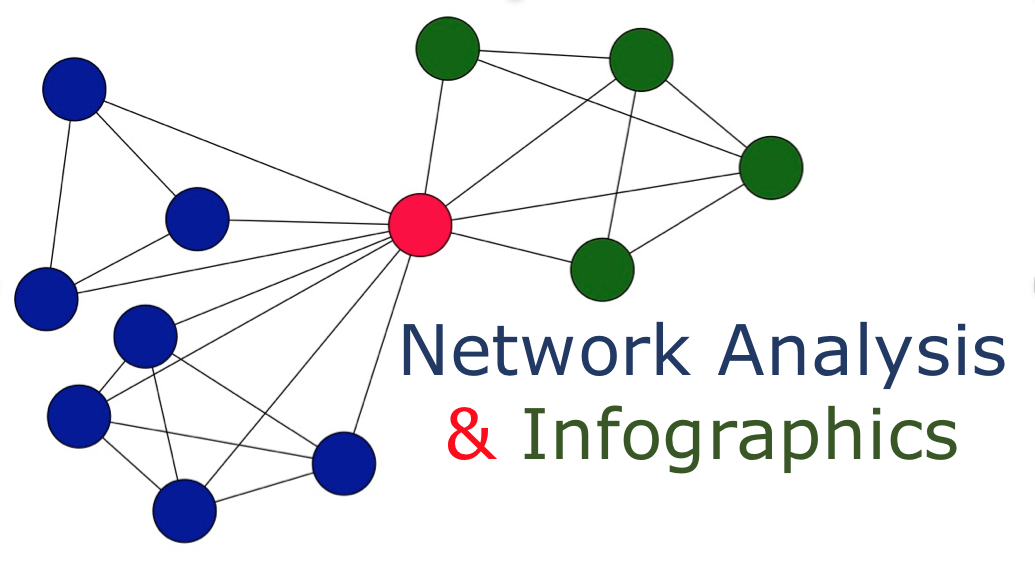
\includegraphics[width=2.5cm]{../_shared_pics/logo}

\medskip

\textit{{\color{dkgreen}{Week 1: 28 January 2022}}}\\
}


\date{} % Date, can be changed to a custom date

\begin{document}

\begin{frame}
\titlepage % Print the title page as the first slide

\begin{textblock*}{10pt}(0pt, 0.9\textheight)

\includegraphics[width=4cm]{../_shared_pics/SPRU.png}
\end{textblock*}

\end{frame}




%=======================================================
%	Learning outcomes
%=======================================================


\begin{frame}
\frametitle{\insertsection}
\framesubtitle{Learning Outcomes}

\centering
\begin{tabular}{lp{5.5cm}l}
\toprule
\multicolumn{2}{l}{\textbf{Learning outcome}} & \textbf{Assessment mode}\\
\hline
\\
\rowcolor{green!20}1 & 
Explain the concept of network and list the main network indicators & 
ESS\\
\\
2 & 
Describe and apply the major techniques for the collection of network data and their statistical analysis & 
ESS, GPN + GWS\\
\\
3 & 
Identify the main characteristics of networks by means of network measures  & 
ESS, GPN + GWS\\
\\
4 &
Employ network analysis techniques to produce network data-based infographics & 
GPN + GWS\\
\\
\bottomrule
\multicolumn{3}{l}{\scriptsize Note: ESS: Essay; GPN: Group Presentation; GWS: Group Written Submission}\\
\end{tabular}

\end{frame}

%------------------------------------------------



%=======================================================
%	Intro slides
%=======================================================

\begin{frame}
\frametitle{Overview}
\tableofcontents[hideallsubsections]
\end{frame}

%-----------------------------------


%=======================================================
%	Old school exercise
%=======================================================

\section{The `old school' exercise}

%-----------------------------------

\bgroup
\setbeamercolor{background canvas}{bg = navyblue}
\begin{frame}[plain]{}
\begin{center}
\color{white}{\Huge\insertsection}
\end{center}
\end{frame}
\egroup

%-----------------------------------

\begin{frame}
\frametitle{\insertsection}

\begin{columns}[c]
\column{.75\textwidth}
You are provided with a list 20 {\color{blue}{R\&D projects}}. These projects involve different {\color{blue}{types of organisations}}. You are requested to:

\medskip

\begin{enumerate}
\item Draw a network the depicts the collaboration activity of firms on projects (inter-organisational network)

\medskip

\item Which are the most influential organisations in this network?

\medskip

\item Which are the most critical organisations for the cohesion of the network?

\medskip

\item Upload a picture of your network \\
	\url{https://padlet.com/yaslan2/oysry42vouhcetvt}
	
\end{enumerate}


\column{.25\textwidth}

\centering
\scriptsize
\begin{table}
\begin{tabular}{cl}
\bottomrule
\textbf{R\&D project} & \textbf{List of partners}\\
\hline
Proj01          & U2, F1, NG1\\
Proj02          & U1, NG4, F1\\
Proj03          & NG3, NG1, F1\\
Proj04          & NG3, NG4, F1\\
Proj05          & U3, F1\\
Proj06          & U3, F2\\
Proj07          & U3, F3\\
Proj08          & U3, U4\\
Proj09          & F1\\
Proj10          & U5\\
Proj11          & U4, U5, U6\\
Proj12          & U3, U7\\
Proj13          & U7, G1\\
Proj14          & U7, O1\\
Proj15          & U7, G2\\
Proj16          & G2, F3\\
Proj17          & F3, O2\\
Proj18          & O2, F4, NG2\\
Proj19          & F4, U9, NG2\\
Proj20          & NG2, U8\\
\bottomrule
\multicolumn{2}{l}{\tiny Firm (F); University (U);}\\
\multicolumn{2}{l}{\tiny Gov. (G); Non-Gov. (NG);}\\
\multicolumn{2}{l}{\tiny Other (O)}
\end{tabular}
\end{table}

\end{columns}
   
\end{frame}

%-----------------------------------

\begin{frame}
\frametitle{\insertsection}
    
\centering
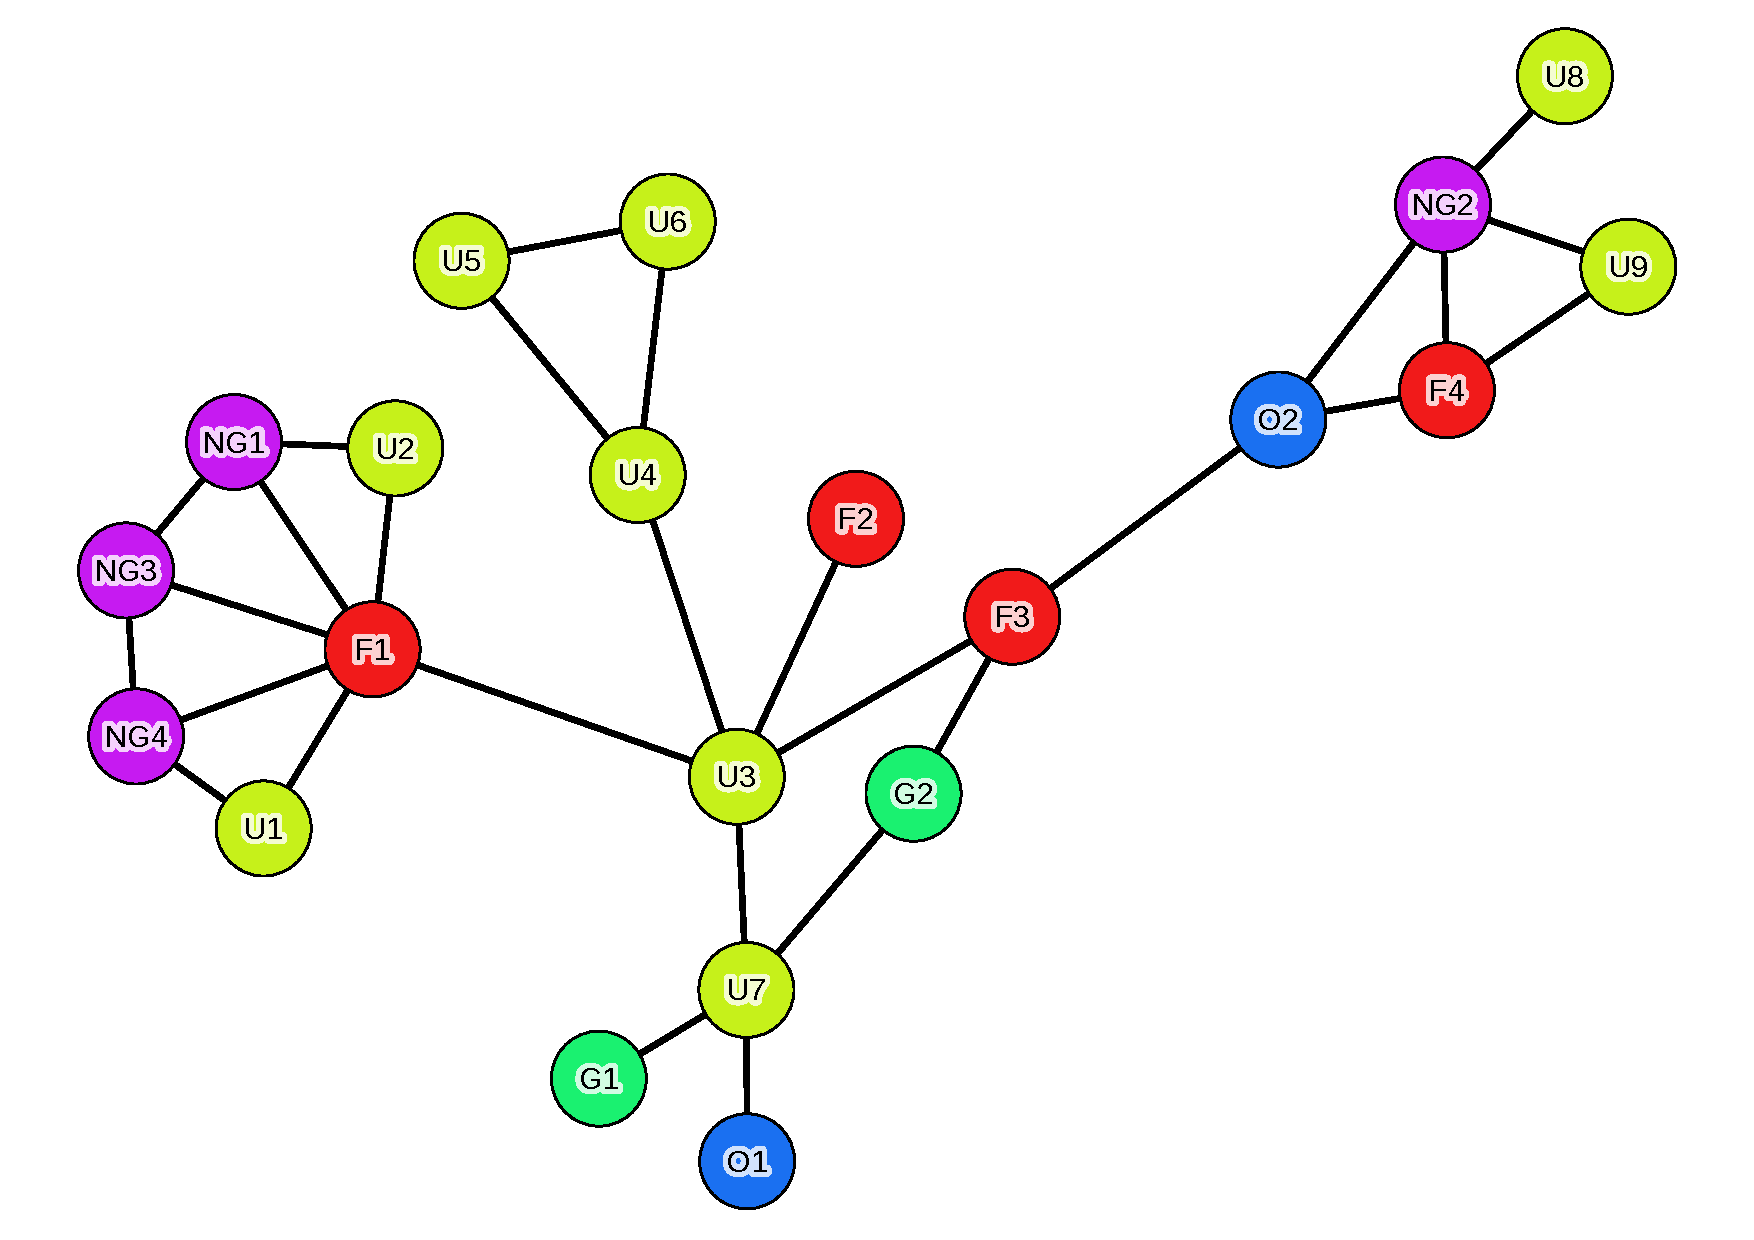
\includegraphics[width=0.9\linewidth,height=\textheight,keepaspectratio]{exercise_gephi}
     
\end{frame}

%-----------------------------------

%-----------------------------------

\begin{frame}
\frametitle{\insertsection}
    
\centering
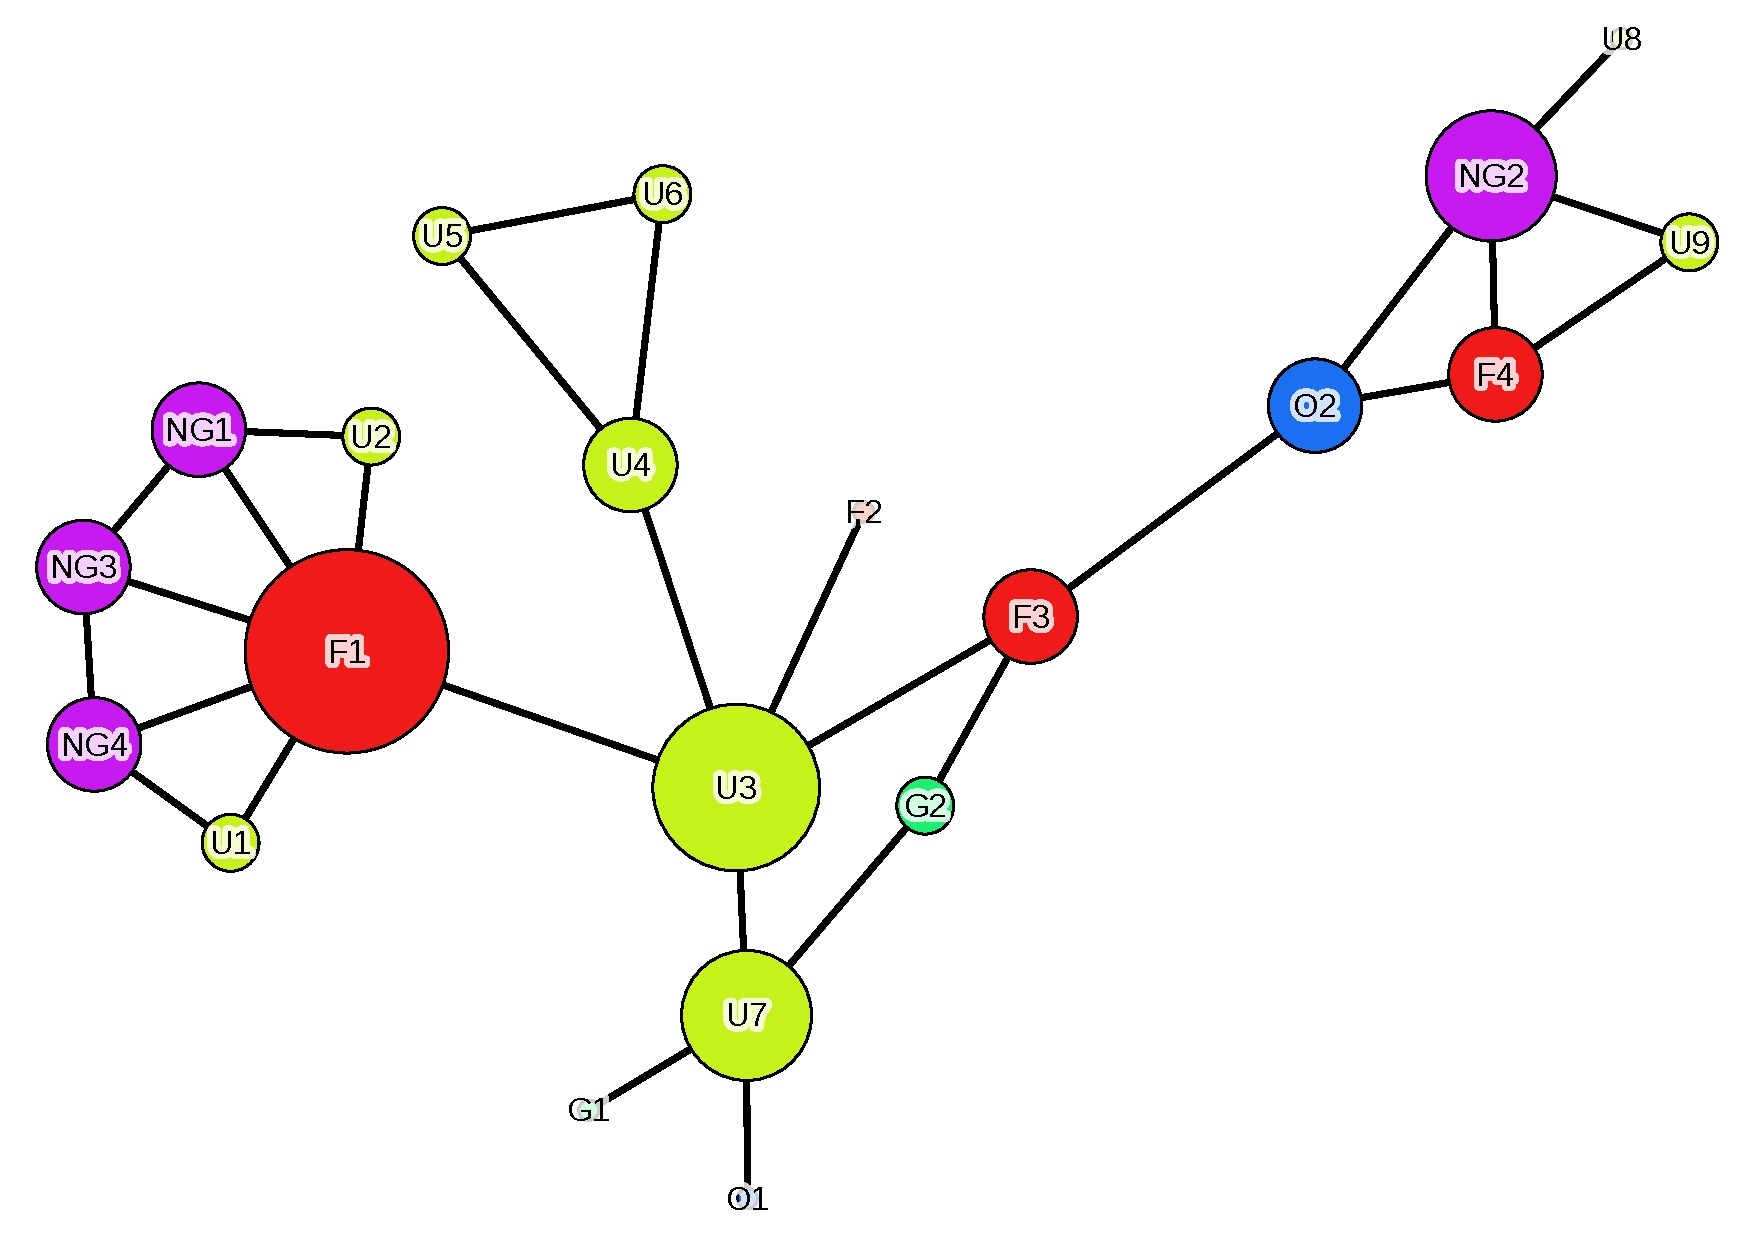
\includegraphics[width=0.9\linewidth,height=\textheight,keepaspectratio]{exercise_degree_gephi}
     
\end{frame}

%-----------------------------------


%-----------------------------------

\begin{frame}
\frametitle{\insertsection}
    
\centering
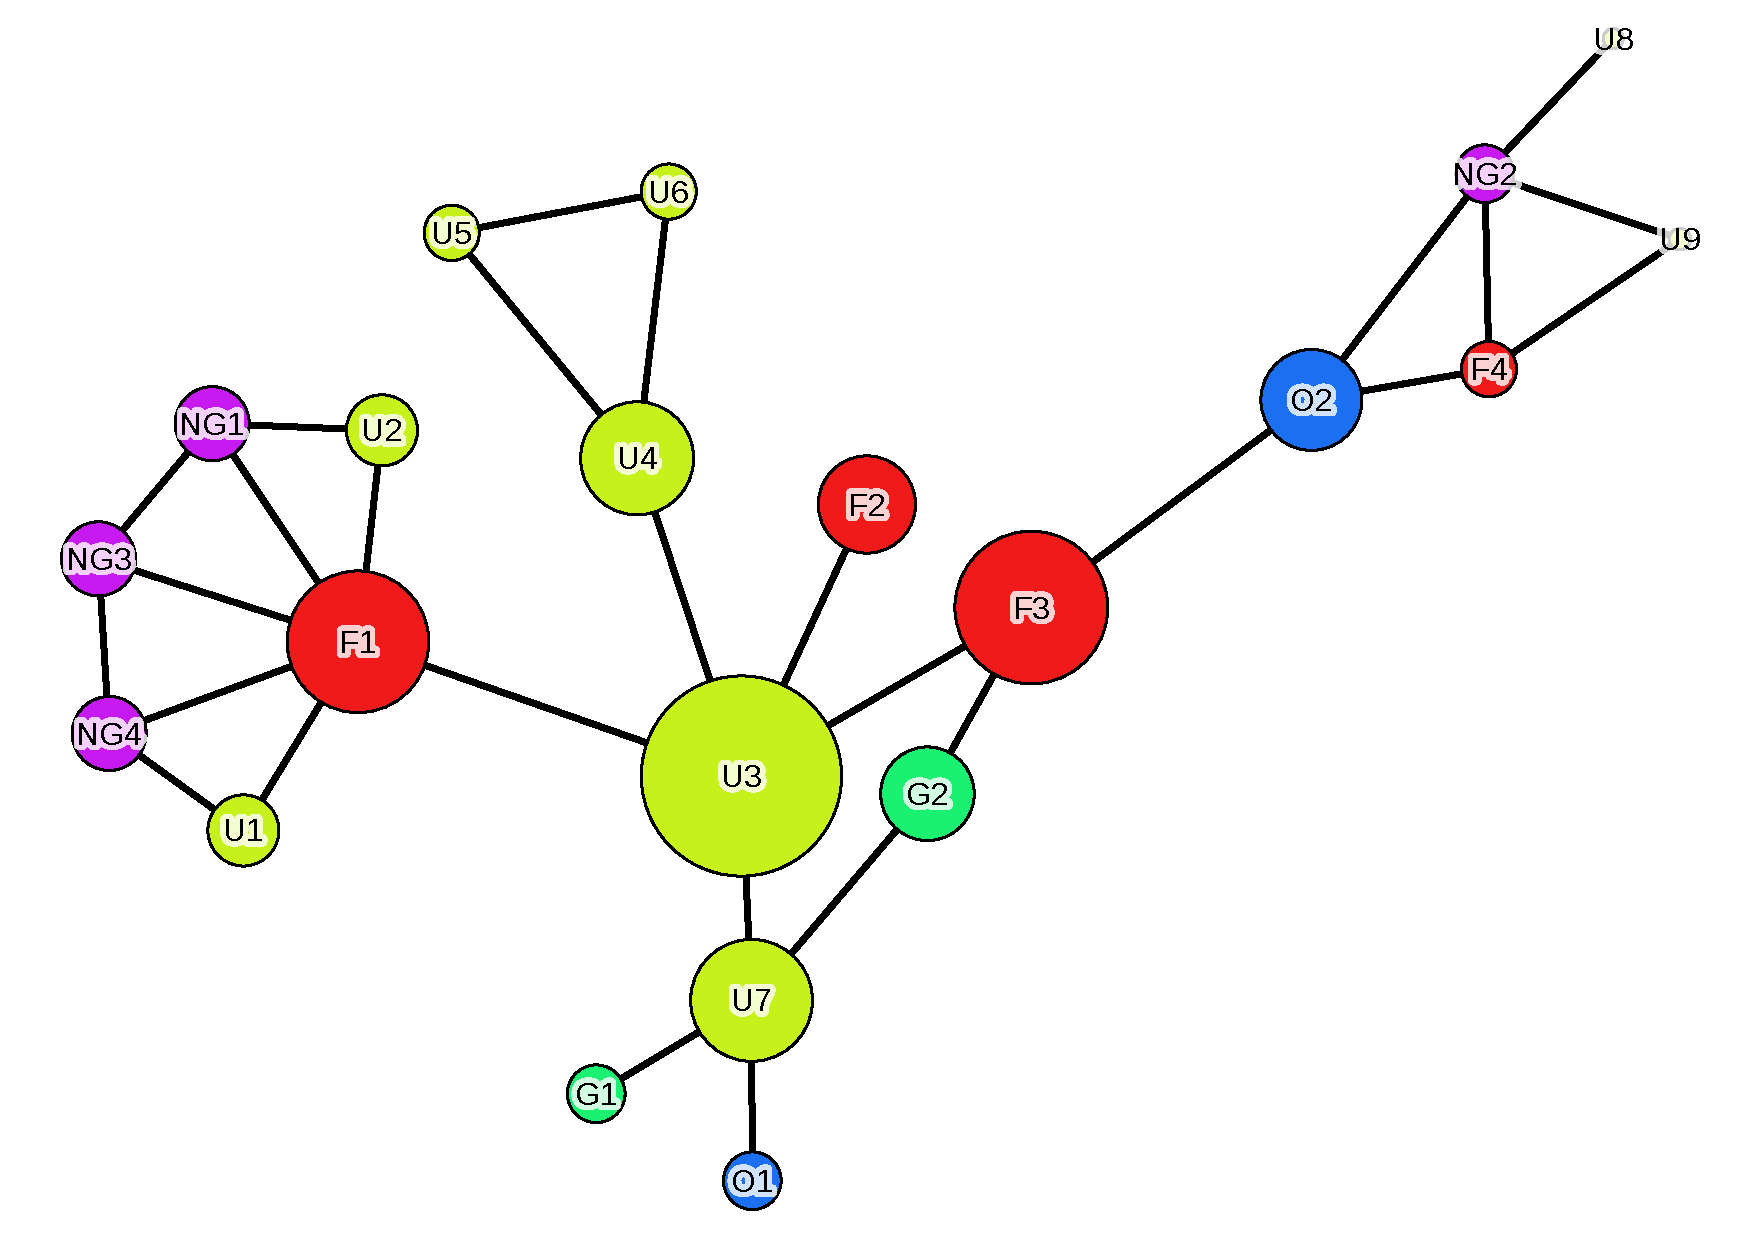
\includegraphics[width=0.9\linewidth,height=\textheight,keepaspectratio]{exercise_closeness_gephi}
     
\end{frame}

%-----------------------------------


%-----------------------------------

\begin{frame}
\frametitle{\insertsection}
    
\centering
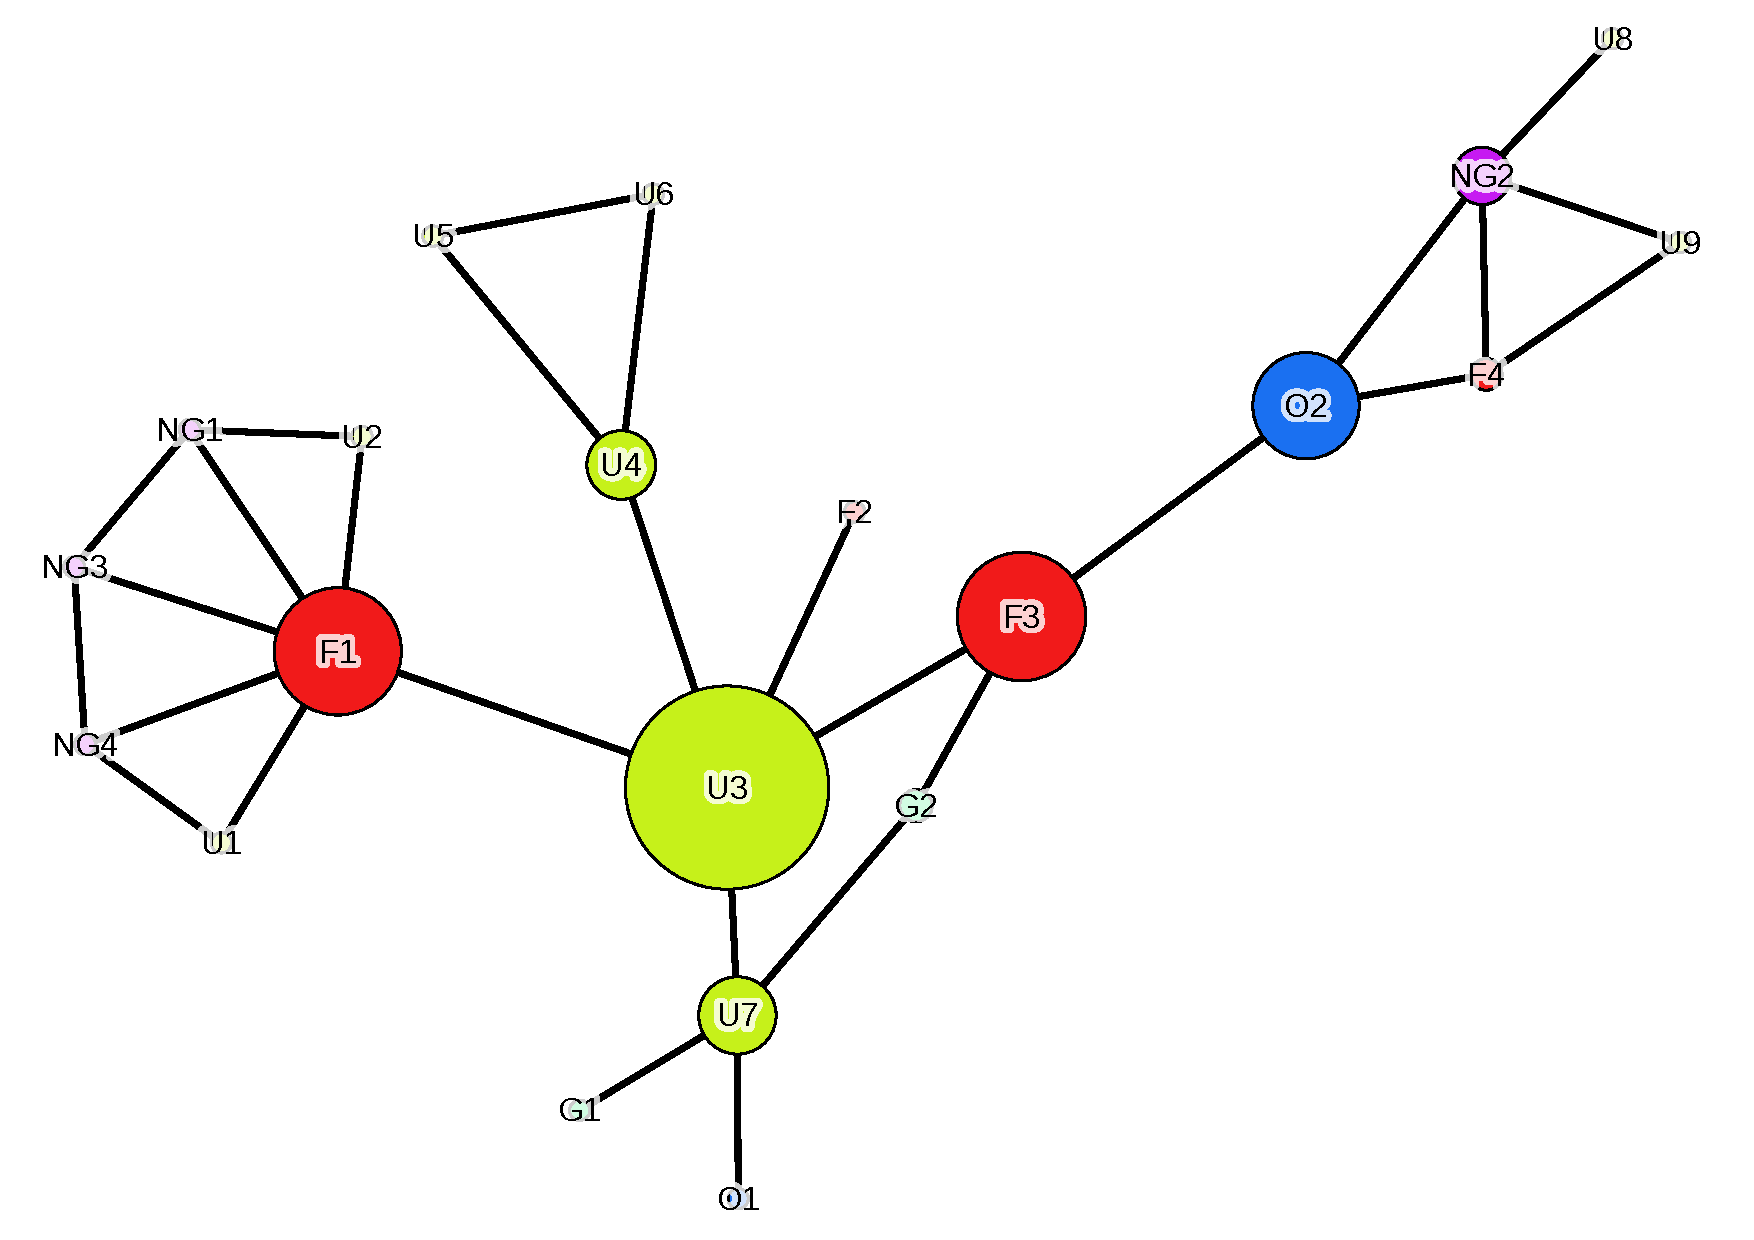
\includegraphics[width=0.9\linewidth,height=\textheight,keepaspectratio]{exercise_betweenness_gephi}
     
\end{frame}

%-----------------------------------

%-----------------------------------

\begin{frame}
\frametitle{\insertsection}
\framesubtitle{Degree centrality}

\begin{columns}[c]
\column{.70\textwidth}
    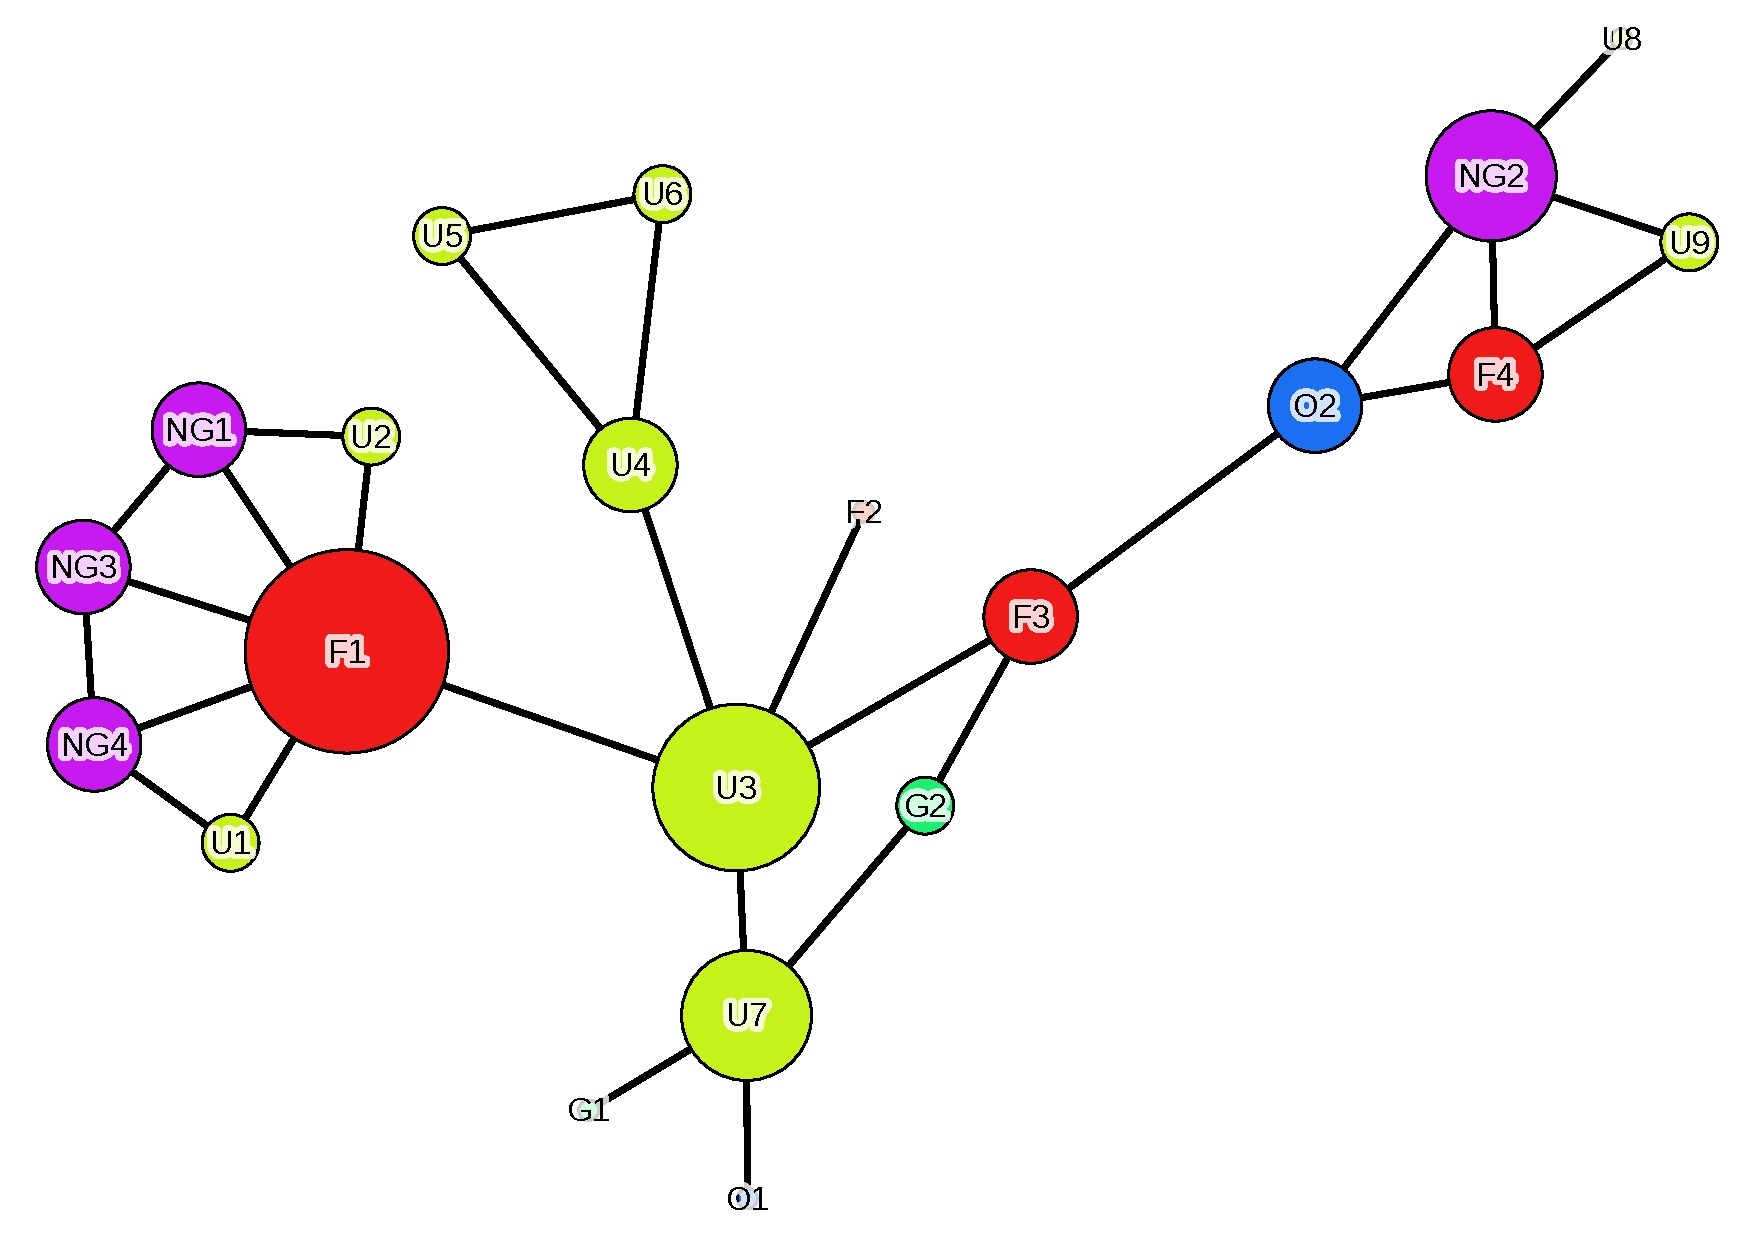
\includegraphics[width=\linewidth,height=\textheight,keepaspectratio]{exercise_degree_gephi}

\column{.30\textwidth}
\centering
\scriptsize
\begin{table}
\centering
\begin{tabular}{cc}
\bottomrule 
Node & $C_{D}(n_{i})$ \\
\hline
F1   & 6      \\
F2   & 1      \\
F3   & 3      \\
F4   & 3      \\
G1   & 1      \\
G2   & 2      \\
NG1  & 3      \\
NG2  & 4      \\
NG3  & 3      \\
NG4  & 3      \\
O1   & 1      \\
O2   & 3      \\
U1   & 2      \\
U2   & 2      \\
U3   & 5      \\
U4   & 3      \\
U5   & 2      \\
U6   & 2      \\
U7   & 4      \\
U8   & 1      \\
U9   & 2   \\
\bottomrule   
\end{tabular}
\end{table}
\end{columns}
   
\end{frame}

%-----------------------------------

\begin{frame}
\frametitle{\insertsection}
\framesubtitle{Closeness centrality}

\begin{columns}[c]
\column{.70\textwidth}
    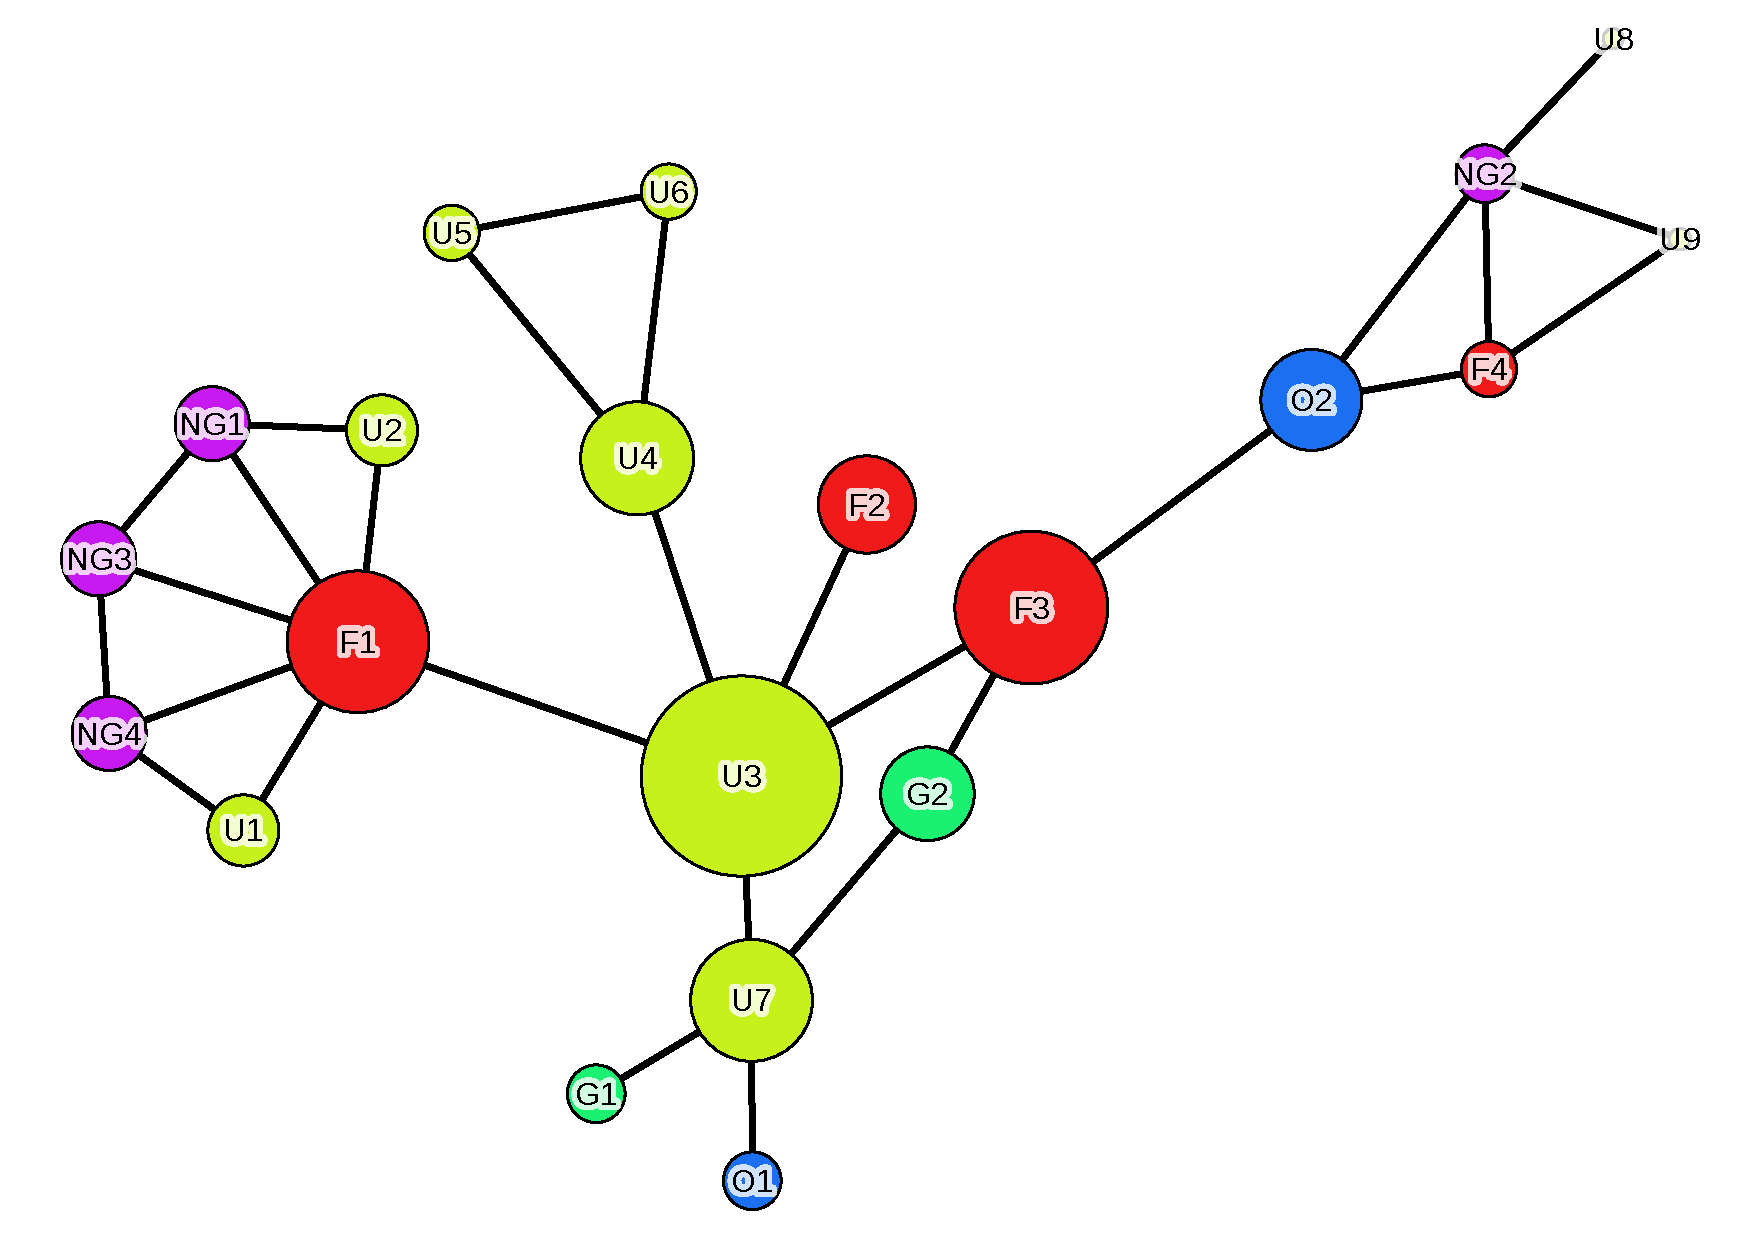
\includegraphics[width=\linewidth,height=\textheight,keepaspectratio]{exercise_closeness_gephi}

\column{.30\textwidth}
\centering
\scriptsize
\begin{table}
\centering
\begin{tabular}{cc}
\bottomrule 
Node & $C_{C}(n_{i})$ \\
\hline
F1   & 0.40       \\
F2   & 0.33      \\
F3   & 0.42      \\
F4   & 0.27      \\
G1   & 0.27      \\
G2   & 0.33      \\
NG1  & 0.30       \\
NG2  & 0.27      \\
NG3  & 0.30       \\
NG4  & 0.30       \\
O1   & 0.27      \\
O2   & 0.34      \\
U1   & 0.29      \\
U2   & 0.29      \\
U3   & 0.49      \\
U4   & 0.36      \\
U5   & 0.27      \\
U6   & 0.27      \\
U7   & 0.37      \\
U8   & 0.22      \\
U9   & 0.22    \\
\bottomrule   
\end{tabular}
\end{table}
\end{columns}
   
\end{frame}

%-----------------------------------

\begin{frame}
\frametitle{\insertsection}
\framesubtitle{Betweenness centrality}

\begin{columns}[c]
\column{.70\textwidth}
    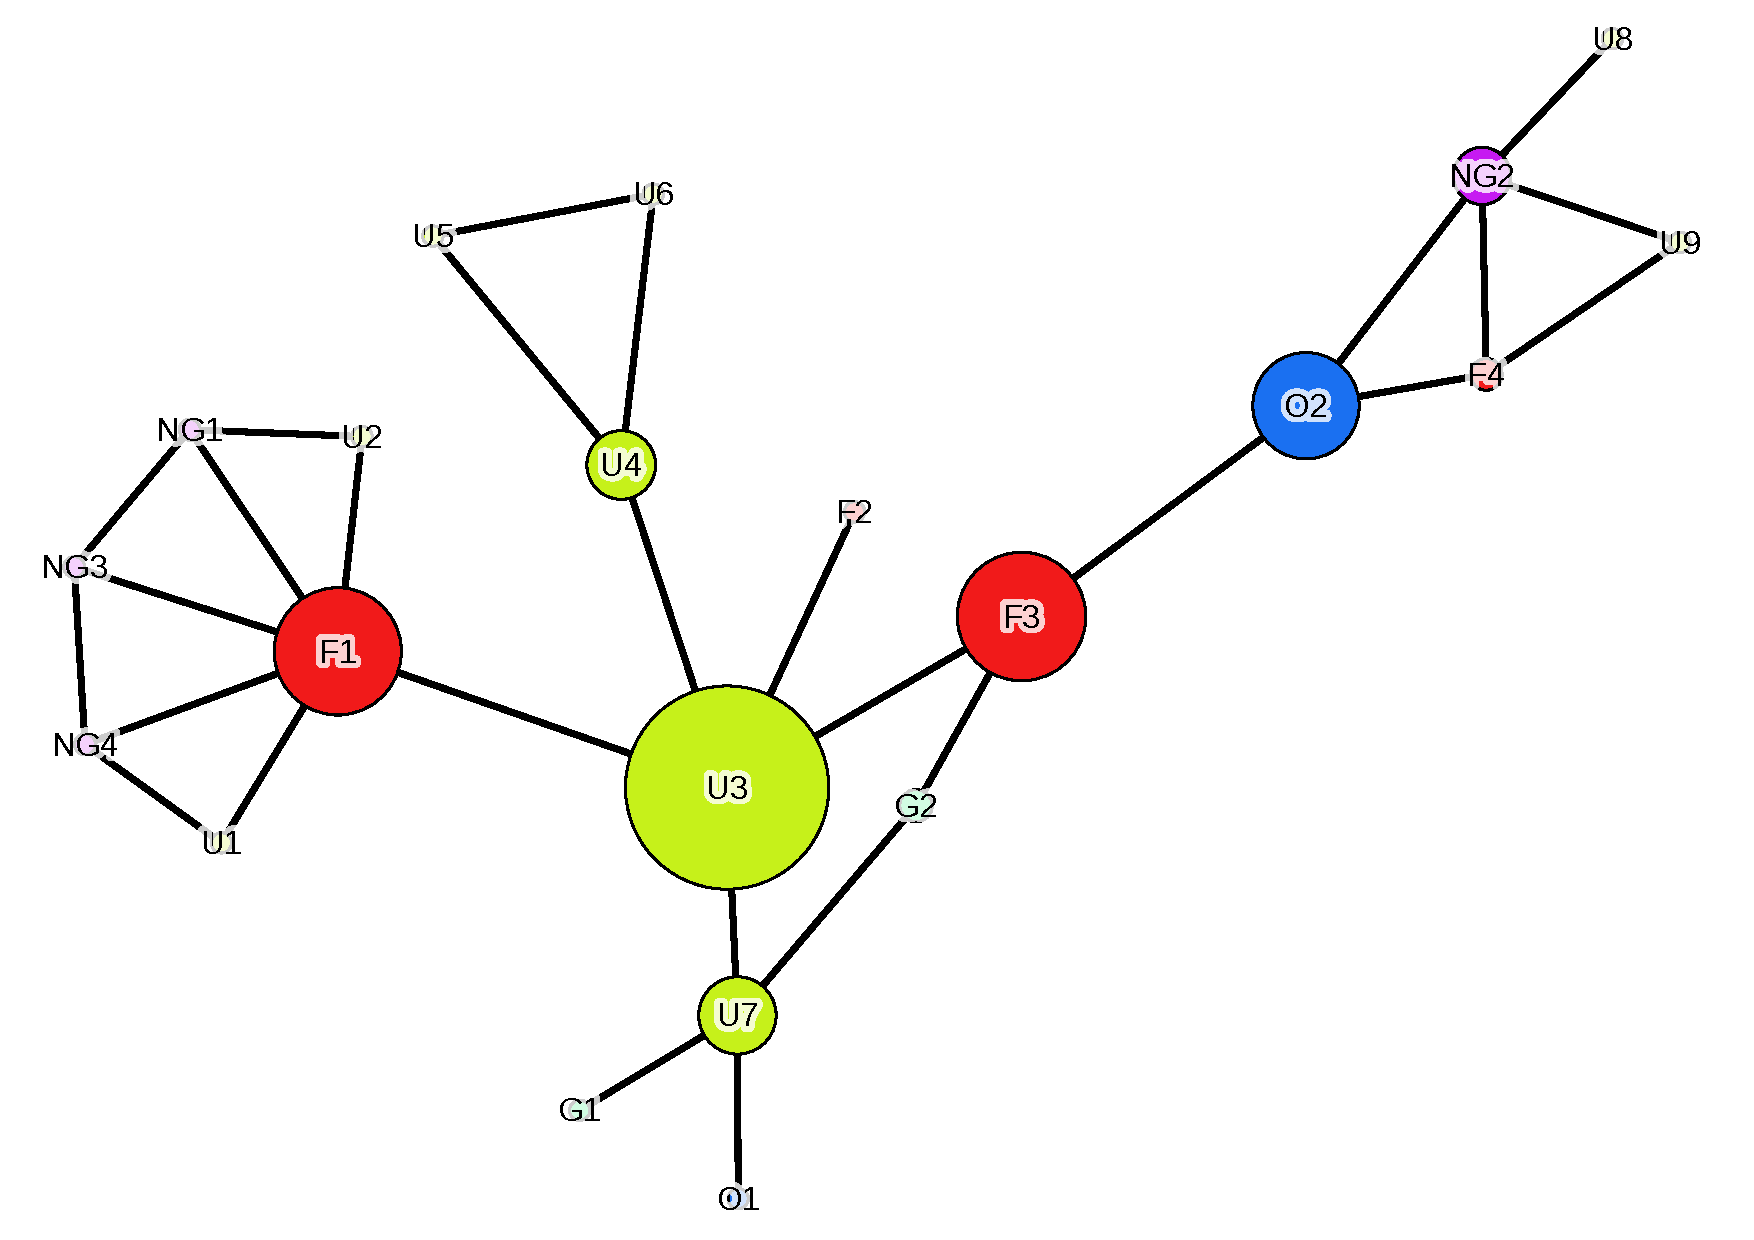
\includegraphics[width=\linewidth,height=\textheight,keepaspectratio]{exercise_betweenness_gephi}

\column{.30\textwidth}
\centering
\scriptsize
\begin{table}
\centering
\begin{tabular}{cc}
\bottomrule 
Node & $C_{B}(n_{i})$ \\
\hline
F1   & 0.42        \\
F2   & -           \\
F3   & 0.42        \\
F4   & 0.04        \\
G1   & -           \\
G2   & 0.05        \\
NG1  & 0.00           \\
NG2  & 0.14        \\
NG3  & 0.00           \\
NG4  & 0.00           \\
O1   & -           \\
O2   & 0.34        \\
U1   & -           \\
U2   & -           \\
U3   & 0.72        \\
U4   & 0.19        \\
U5   & -           \\
U6   & -           \\
U7   & 0.22        \\
U8   & -           \\
U9   & -          \\
\bottomrule   
\end{tabular}
\end{table}
\end{columns}
   
\end{frame}

%-----------------------------------







%=======================================================
% R, RStudio, and igraph
%=======================================================
\section{R, RStudio, and igraph}

%-----------------------------------

\bgroup
\setbeamercolor{background canvas}{bg = navyblue}
\begin{frame}[plain]{}
\begin{center}
\color{white}{\Huge\insertsection}
\end{center}
\end{frame}
\egroup

%-----------------------------------


\begin{frame}
\frametitle{\insertsection}

\begin{center}
    
\includegraphics[height=1.5cm]{../_shared_pics/r_logo}\\
    \url{www.r-project.org}
\end{center}

\medskip
\medskip

\begin{itemize}[<+->]
\item A {\color{blue}{language}} and  {\color{blue}{environment}} for statistical computing and graphics
\item Runs on Windows, Linux, macOS
\item Initially developed for {\color{blue}{statistical analysis}} by Robert Gentleman and Ross Ihaka (University of Auckland) -- that's why ``R''.
\item {\color{blue}{Core Group}} with write access to the R source
\item Constantly updated and with access to {\color{blue}{~19,000 packages}} (January 2022, \url{www.r-pkg.org})
\end{itemize}

\end{frame}

%-----------------------------------

\begin{frame}
\frametitle{\insertsection}


\includegraphics[height=0.5cm]{../_shared_pics/r_logo}\\
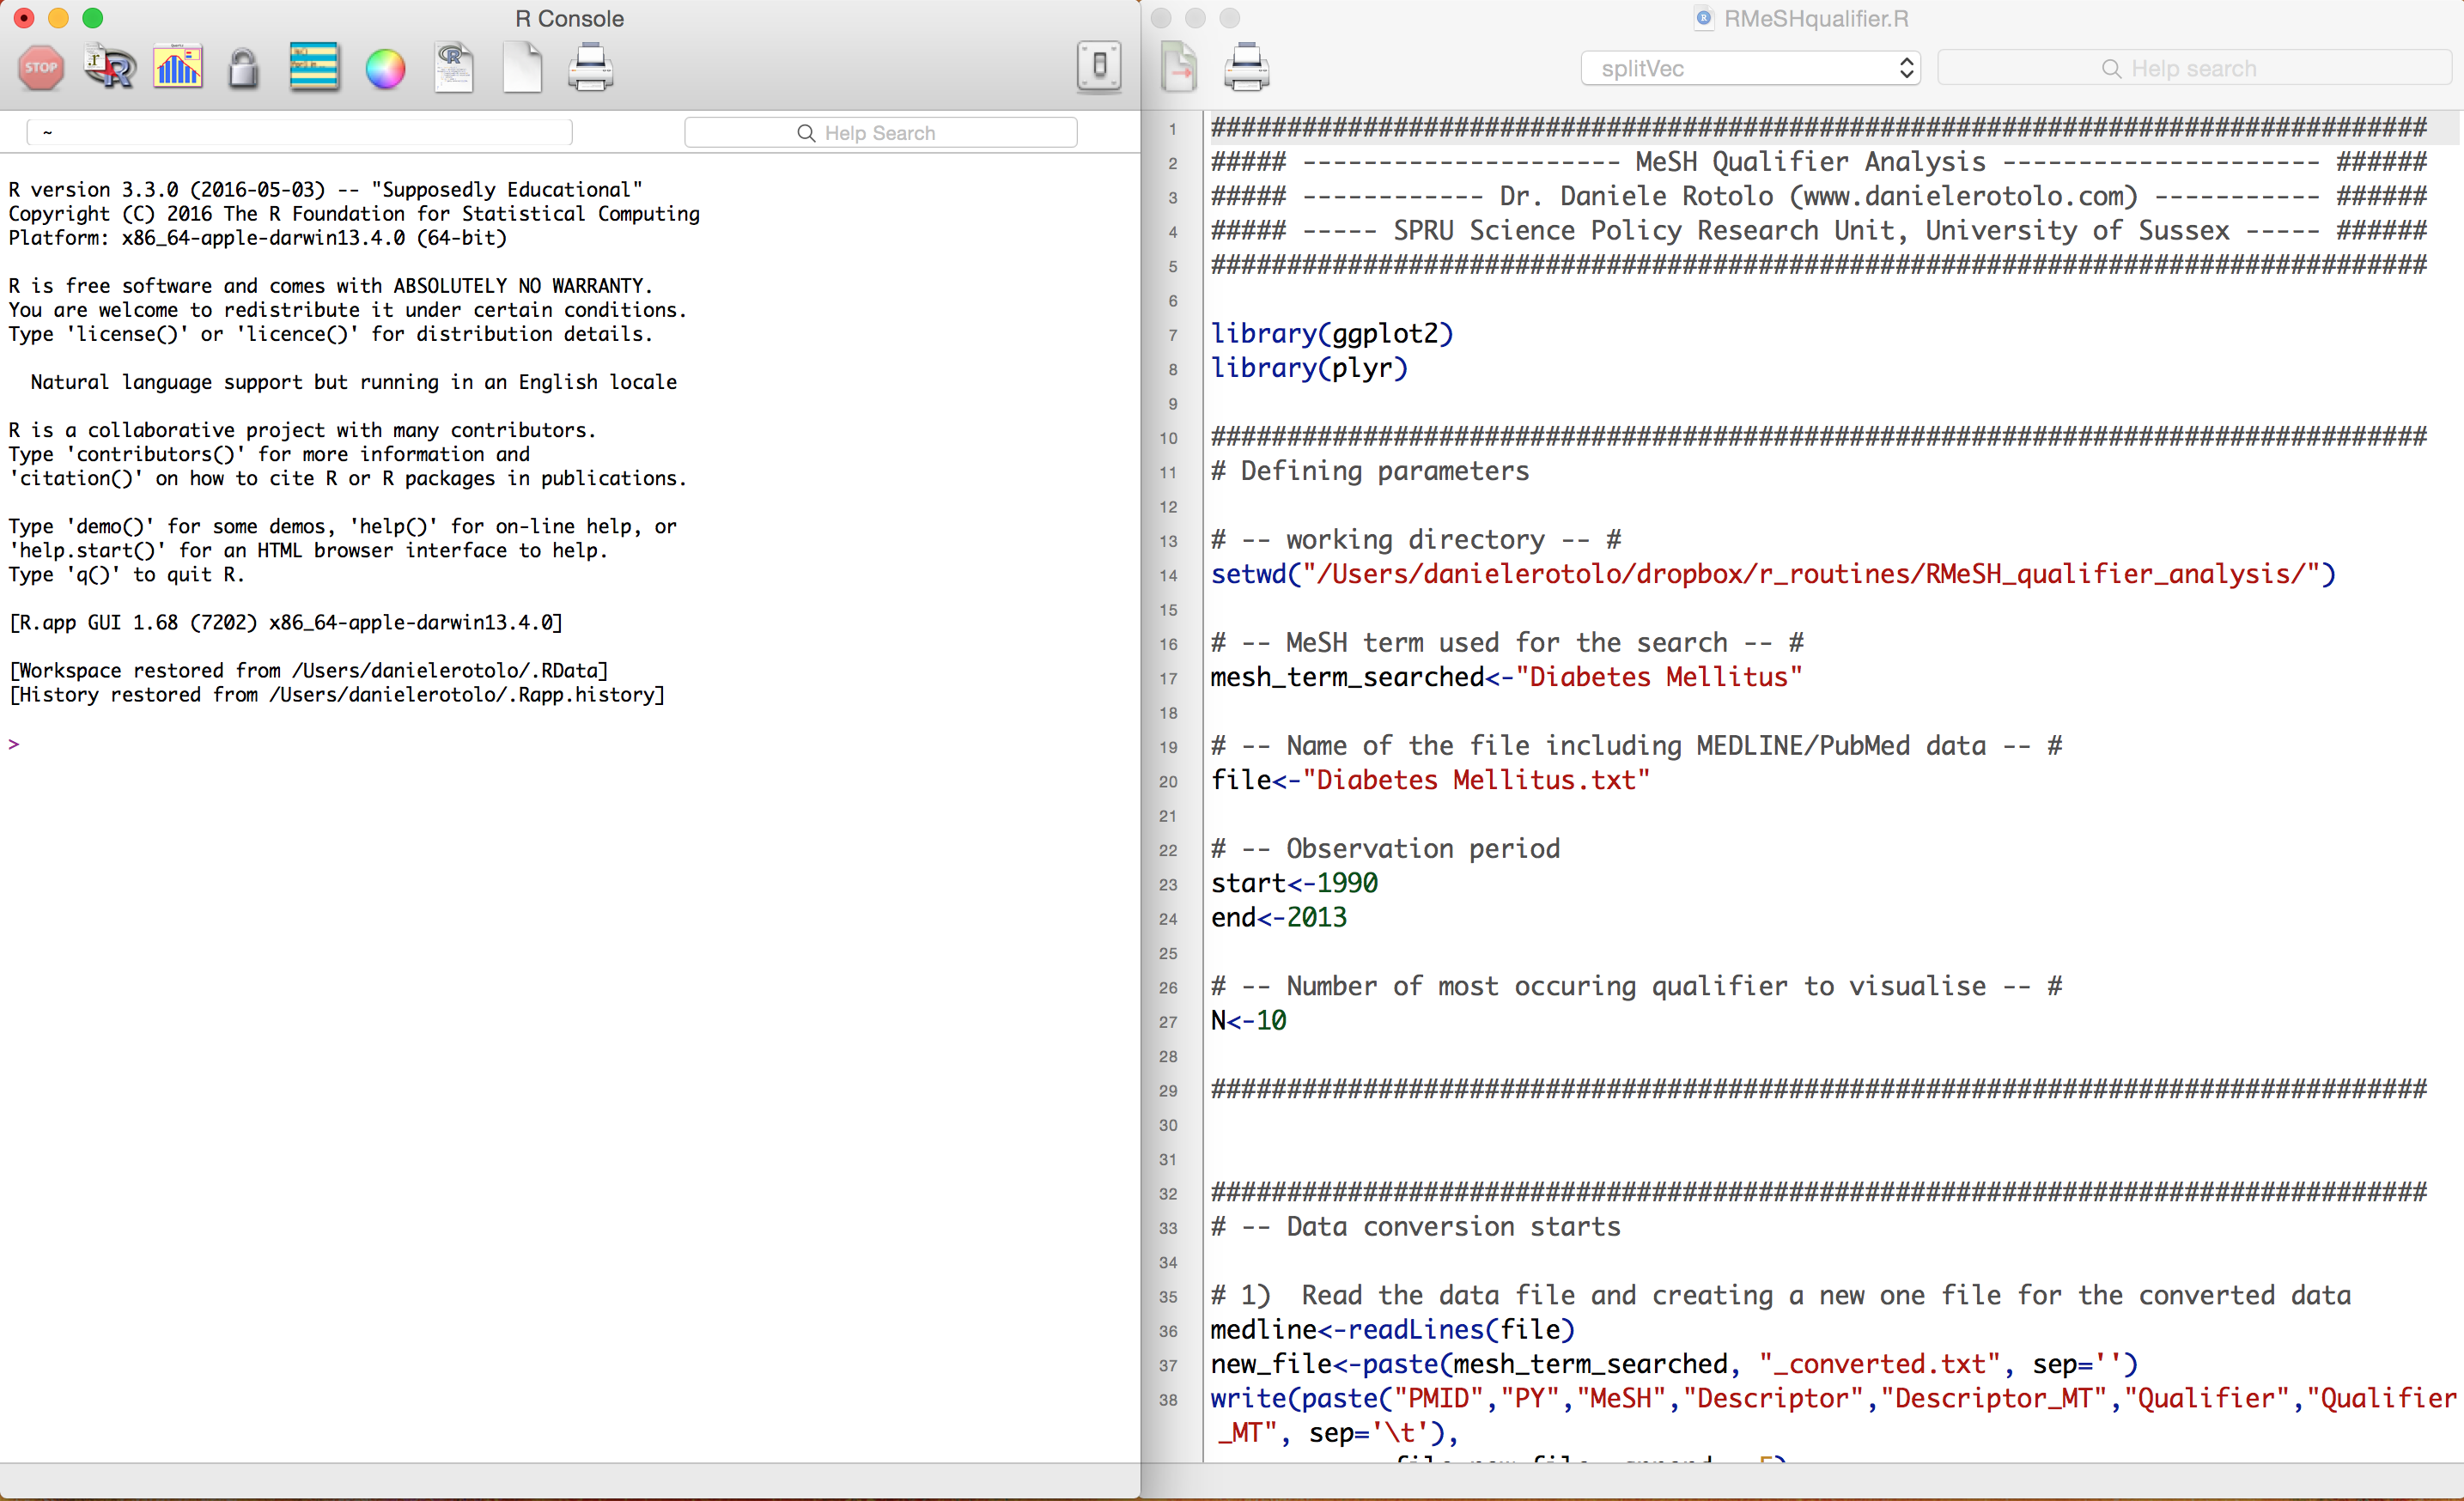
\includegraphics[width=\linewidth,frame]{r_interface}

\end{frame}

%-----------------------------------

\begin{frame}
\frametitle{\insertsection}

\begin{center}
    
\includegraphics[height=1.5cm]{../_shared_pics/rstudio_logo}\\
    \url{www.rstudio.com}
\end{center}

\medskip
\medskip

\begin{itemize}[<+->]
\item An {\color{blue}{open-source editor}} for R 
\item Developed by a company called RStudio
\item {\color{blue}{Functionalities}} that are otherwise not available in the standard R editor
\item Support, tutorials, webinars 

\end{itemize}

\end{frame}

%-----------------------------------

\begin{frame}
\frametitle{\insertsection}


\includegraphics[height=0.5cm]{../_shared_pics/rstudio_logo}\\
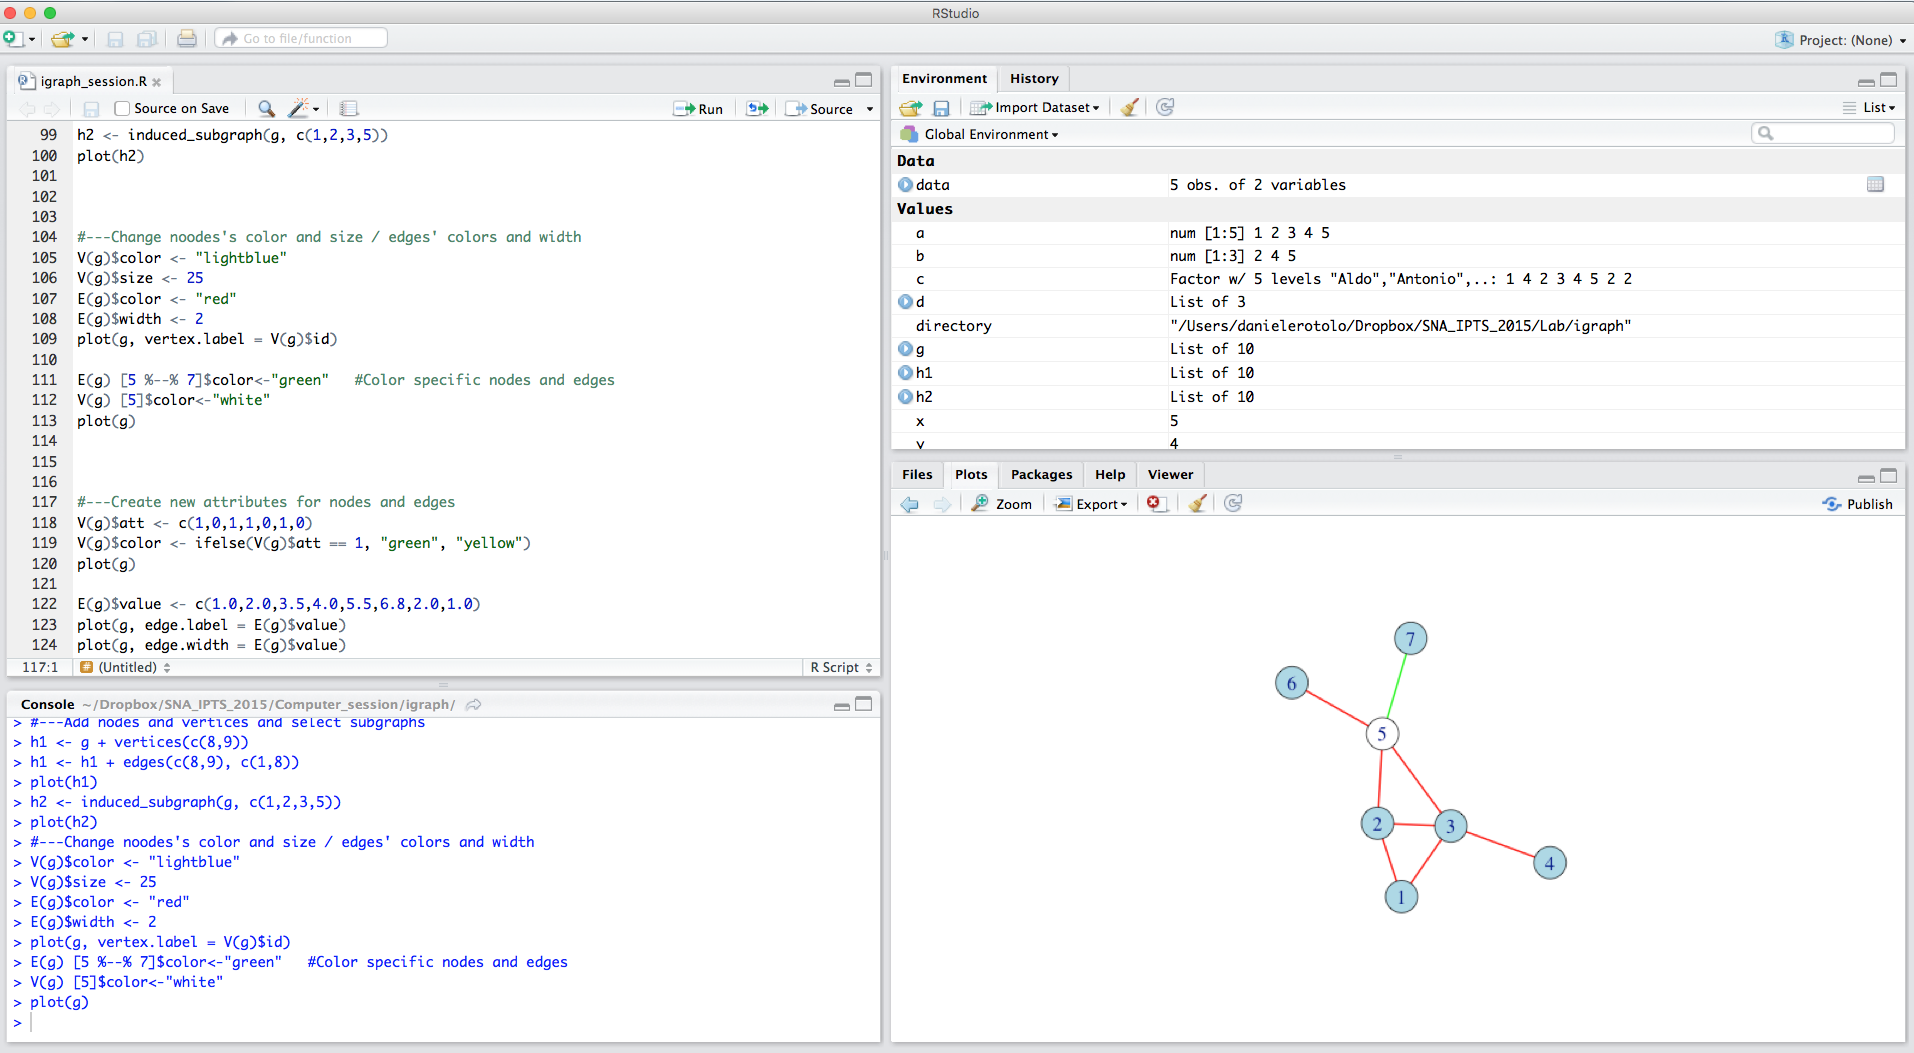
\includegraphics[width=\linewidth,frame]{rstudio_interface}

\end{frame}

%-----------------------------------

\begin{frame}
\frametitle{\insertsection}

Elements of the interface:
\begin{itemize}
\item {\color{blue}{Script:}} the list of commands we want R to execute
\item {\color{blue}{Console:}} the list of commands R executes and the outcomes of these
\item {\color{blue}{Environment, History:}} variables, datasets, and  executed commands
\item {\color{blue}{Files, Plot, Packages, Help, Viewer:}} generated charts, loaded packages, etc.
\end{itemize}

\end{frame}

%-----------------------------------

\begin{frame}
\frametitle{\insertsection}

\begin{center}
    
\includegraphics[height=1.5cm]{../_shared_pics/igraph_logo}\\
    \url{http://igraph.org/r/}
\end{center}

\begin{itemize}[<+->]
\item Provides a relatively comprehensive {\color{blue}{set of tools to perform network analysis}}
\item Developed by G\'{a}bor Cs\'{a}rdi (Harvard University) and others
\item Excellent textbook \cite{Kolaczyk2014}
\end{itemize}

\end{frame}

%-----------------------------------





%=======================================================
%	Ready ...?
%=======================================================
\section{Ready ...?}

%-----------------------------------

\bgroup
\setbeamercolor{background canvas}{bg = navyblue}
\begin{frame}[plain]{}
\begin{center}
\color{white}{\Huge\insertsection}
\end{center}
\end{frame}
\egroup

%-----------------------------------

\begin{frame}
\frametitle{\insertsection}
\framesubtitle{R and RStudio}


{\color{blue}{On campus*}}
\begin{enumerate}
	\item Go to http://rstudio.uscs.susx.ac.uk/
	\item Access the website by using your University of Sussex account
\end{enumerate}

\medskip

{\color{blue}{On your personal computer}}
\begin{enumerate}
	\item Install R
	\item Install RStudio
\end{enumerate}

\medskip

{\color{blue}{RStudio cloud}}
\begin{enumerate}
	\item Go to \url{https://rstudio.cloud}
	\item Register and sign in
\end{enumerate}

\medskip
\medskip

*You can access the server off campus by using remote desktop
http://www.sussex.ac.uk/its/services/software/windowsremote

\end{frame}

%-----------------------------------

\begin{frame}[fragile]
\frametitle{\insertsection}
\framesubtitle{Installing igraph}

Through the {\color{blue}{RStudio interface}}:\\
\begin{enumerate}
	\item Tools
	\item Install Packages
	\item Search for igraph
	\item Tick the box ``Install Dependencies''
	\item Install
\end{enumerate}
\medskip
\medskip
or\\
\medskip
\medskip
Through the {\color{blue}{RStudio console}}

\begin{lstlisting}[language=R]
install.packages("igraph")
library("igraph")
\end{lstlisting}

\end{frame}

%-----------------------------------


%=======================================================
%	Ready ...?
%=======================================================
\section{Some useful (and freely available) resources to learn R}

%-----------------------------------

\begin{frame}[fragile]
	\frametitle{\insertsection}
\begin{itemize}
	\item \textbf{Books}
		\begin{itemize}
			\item \href{https://r4ds.had.co.nz/}{\underline{\smash{Harley Wickham and Garrett Grolemund - R for Data Science}}}: generic introduction to R and to the data analysis workflow
			\item \href{https://serialmentor.com/dataviz/index.html}{\underline{\smash{Claus O. Wilke - Fundamentals of Data Visualisation}}}: mainly based on \verb|ggplot2|, an R package for data visualisation 
		\end{itemize}
	\medskip
	\item \textbf{Online courses:} a host of possible choices!
		\begin{itemize}
			\item \href{https://education.rstudio.com/learn/}{\underline{\smash{RStudio}}} official learning pathways
			\item \href{https://www.linkedin.com/learning/me}{\underline{\smash{Linkedin Learning}}}
			\item Coursera, EdX...
		\end{itemize}
	\medskip
		\item \textbf{Online communities:} practical solutions to specific issues
		 \begin{itemize}
		 	\item \href{https://stackoverflow.com/questions/tagged/r}{\underline{\smash{StackOverFlow}}} - Q\&A about coding problems
		 	\item \href{https://github.com/}{\underline{\smash{GitHub}}} - a bit more advanced, repository of routines
		 \end{itemize}
	\medskip
	\item \textbf{Twitter:} \#rstats and @rstatstweet

\end{itemize}
\end{frame}






%=======================================================
%	Next time ...
%=======================================================
\section*{Next time ...}

%-----------------------------------

\bgroup
\setbeamercolor{background canvas}{bg = navyblue}
\begin{frame}[plain]{}
\begin{center}
\color{white}{\Huge\insertsection}
\end{center}
\end{frame}
\egroup

%-----------------------------------

\begin{frame}
\frametitle{\insertsection}

\begin{itemize}
\item 	\textbf{Lecture: Network definition}
		\begin{itemize}
		\item Definition of network and different types of networks
		\item Overview of the historical and disciplinary origins of (social) network analysis
		\item Network visualisation standards
		\end{itemize}
\medskip
\medskip
\item 	\textbf{Seminar: Network definition}
		\begin{itemize}
		\item Short intro to R
		\item Basic commands 
		\end{itemize}
\end{itemize}


\end{frame}

%-----------------------------------




%=======================================================
%	Questions
%=======================================================

\section*{Questions}

%-----------------------------------

\bgroup
\setbeamercolor{background canvas}{bg = navyblue}
\begin{frame}[plain]{}
\begin{center}
\color{white}{\Huge\insertsection}
\end{center}
\end{frame}
\egroup

%-----------------------------------



\section*{References}


%-----------------------------------
%	References
%-----------------------------------

\begin{frame}[allowframebreaks]
\frametitle{References}
\tiny
\bibliographystyle{apalike}
\bibliography{../library.bib}
\end{frame}

%---------------------------------------------------------------------------

\end{document}